\documentclass[12pt,a4paper]{article}
\raggedbottom

\usepackage{ugmath}
\usepackage{float}
\usepackage{placeins}
\usepackage[labelfont=bf,labelsep=space]{caption}
\usepackage{pdfpages}
\usepackage{tikz-cd}
\usepackage{amsthm}
\renewcommand{\Tr}{\operatorname{Tr}}
\newcommand{\llaves}[1]{\{#1\}}
\newcommand{\parentesis}[1]{\left(#1\right)}
\newcommand{\corchetes}[1]{\left[#1\right]}
\newcommand{\llavesgrande}[1]{\big\{#1\big\}}
\newcommand{\llavesgrandes}[1]{\left\{#1\right\}}


\begin{document}
        
    \thispagestyle{empty}
    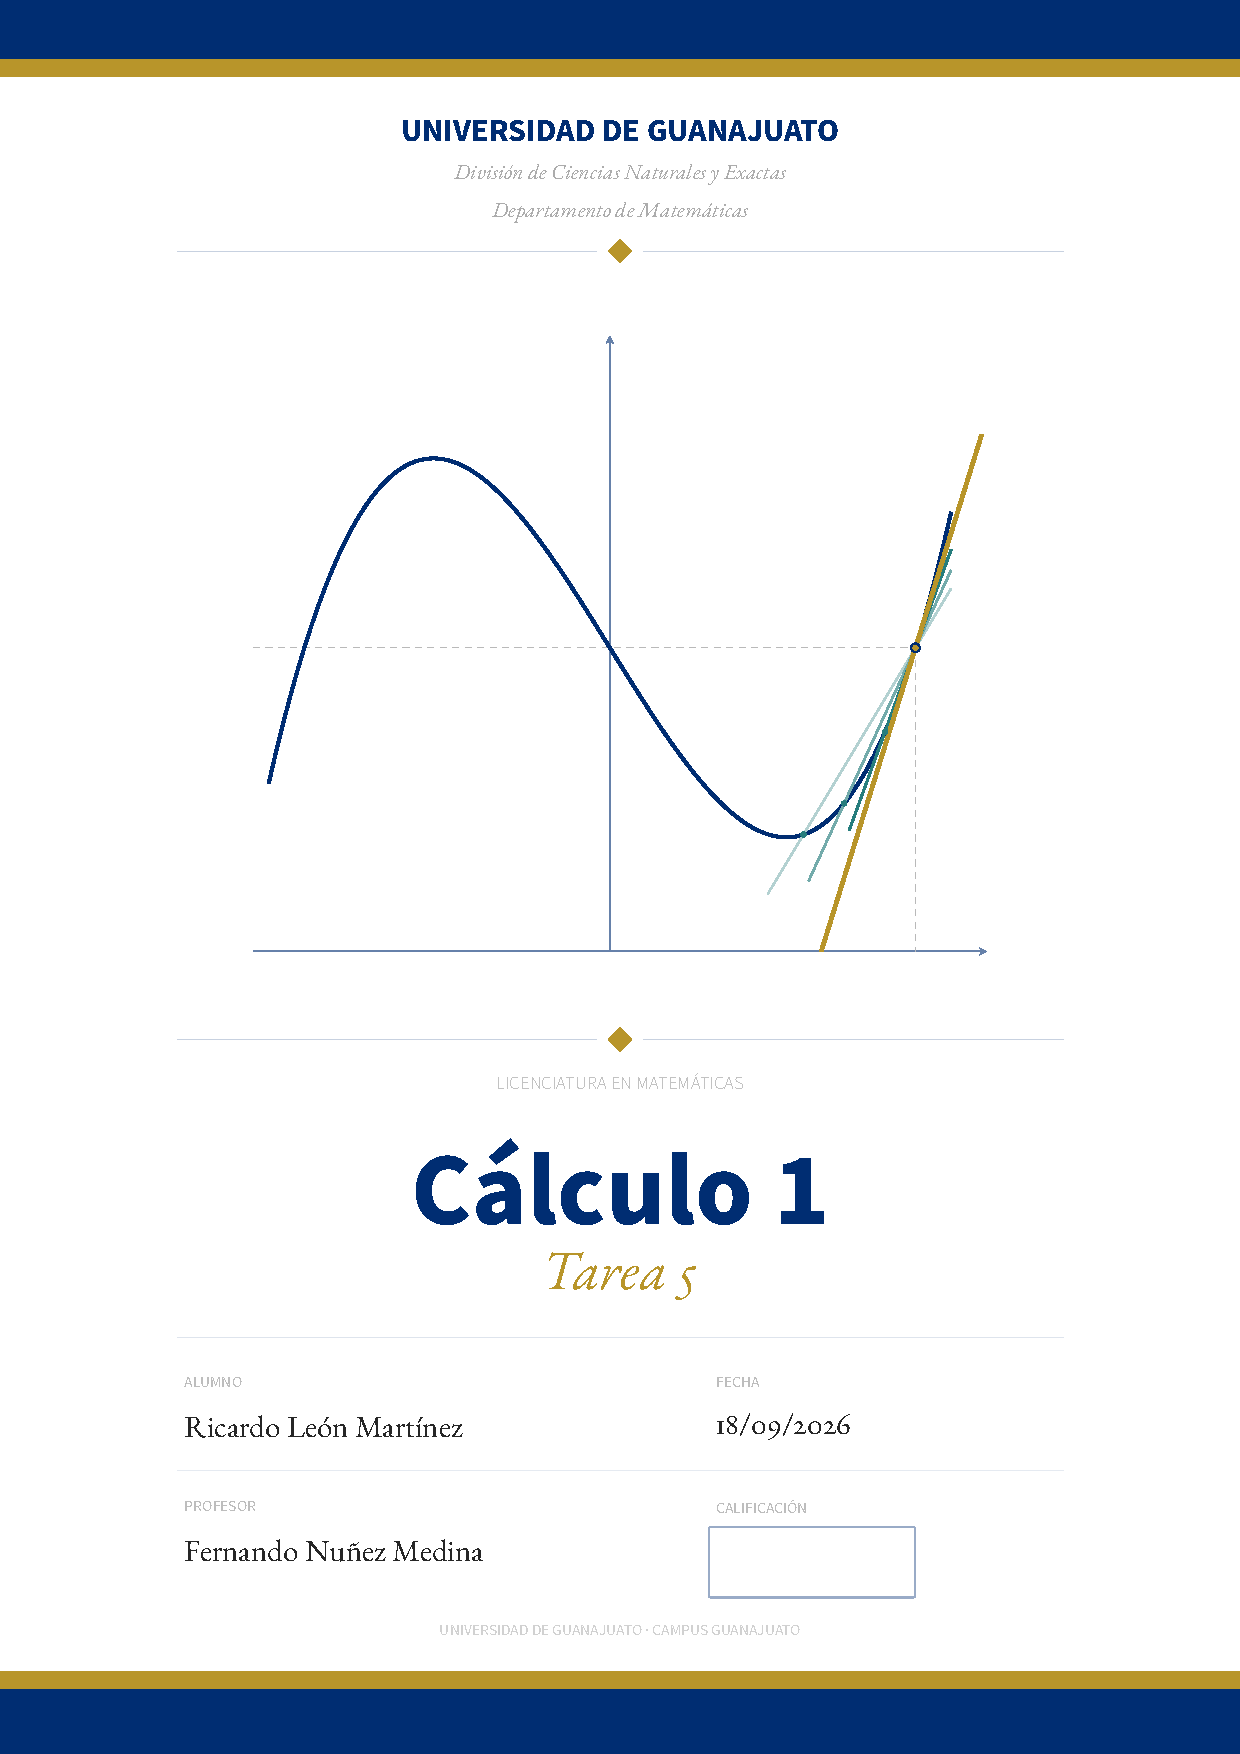
\includepdf[pages=1]{main.pdf}

    \begin{problema}
        Prueba que si $x$
        y $y$ son números reales, con $y\neq0,$ entonces 
        \begin{enumerate}
            \item[(a)] $\frac{+x}{+y}=+\frac{x}{y}.$ \vspace{0.1cm}
            \item[(b)] $\frac{-x}{+y}=-\frac{x}{y}.$ \vspace{0.1cm}
            \item[(c)] $\frac{+x}{-y}=-\frac{x}{y}.$ \vspace{0.1cm}
            \item[(d)] $\frac{-x}{-y}=+\frac{x}{y}.$ 
        \end{enumerate}
        Las leyes de los signos para la división se resumen de manera conveniente
        como 
        \begin{equation*}
            \begin{array}{ccccc}
                + & \text{entre} & + & \text{da} & +\\
                - & \text{entre} & + & \text{da} & -\\
                + & \text{entre} & - & \text{da} & -\\
                - & \text{entre} & - & \text{da} & +
            \end{array}
        \end{equation*}
        \textbf{Sugerencia 1:} El inciso (a) es claro, pues $+x=x,$ $+y=y$
        y $+\left(x/y\right)=x/y.$ Usa la unicidad del inverso aditivo para
        probar los incisos (b) y (c). Finalmente, deduce (d) de los incisos
        (b) y (c). \textbf{Sugerencia 2:} Para probar (b), usa las leyes de
        los signos para la multiplicación, y para probar (c), usa que $\left(-y\right)^{-1}=-\left(y^{-1}\right)$
        y las leyes de los signos para la multiplicación.
    \end{problema}

    \begin{problema}
        Prueba que si $x<y+\e$ para todo $\e>0$, entonces $x\leq y$.
    \end{problema}

    \begin{proof}
        Procedaremos por contradicción. Supongamos que $x>y$. Entonces $x-y>0$. Tomando $\e=x-y$, obtenemos
        \begin{align*}
            x&<y+\e\\
            &=y+x-y\\
            &=x.
        \end{align*}
        Lo cual es una contradicción.
    \end{proof}

    \begin{problema}
        Sean $A$ y $B$ subconjuntos no vacíos de números reales tales que $A\subset B$. Prueba  que
        \begin{equation*}
            \inf(B)\leq\inf(A)\leq\sup(A)\leq\sup(B).
        \end{equation*}
    \end{problema}

    \begin{problema}
        Dados $n$ y $k$ números enteros
        con $0\leq k\leq n$ definimos el \textit{coeficiente binomial} 
        \begin{equation*}
            \binom{n}{k}=\frac{n!}{k!(n-k)!}.
        \end{equation*}
        Recuerda que el número factorial de un número natural $n$ se define
        como $n!=n\cdot\left(n-1\right)\cdots2\cdot1$ y que $0!=1.$ 
        \begin{enumerate}
            \item[(a)]  Sea $n$ un número natural. Prueba que 
            \begin{equation*}
                \binom{n}{0}=\binom{n}{n}=1.
            \end{equation*}
            \item[(b)]  Sean $n$ y $k$ números naturales con $k\leq n.$ Prueba que 
            \begin{equation*}
                \binom{n}{k-1}+\binom{n}{k}=\binom{n+1}{k}.
            \end{equation*}
        \end{enumerate}
    \end{problema}

    \begin{problema}
        Prueba, mediante contraejemplos, que es falso que la suma, resta, producto y cociente de números irracionales sea un número irracional.
    \end{problema}

    \begin{problema}
        Sean $f:A\rightarrow B$ y $C\subset B.$ Definimos la \textit{imagen
        inversa} \index{imagen inversa de un conjunto bajo una función} del
        conjunto $C$ bajo la función $f$ como el conjunto 
        \begin{equation*}
            f^{-1}\left(C\right)=\left\{ x\in A:f\left(x\right)\in C\right\} .
        \end{equation*}
        Dados $C,D\subset B,$ prueba lo siguiente:
        \begin{enumerate}
            \item[(a)] $f^{-1}\left(C\cup D\right)=f^{-1}\left(C\right)\cup f^{-1}\left(D\right).$
            \item[(b)] $f^{-1}\left(C\cap D\right)=f^{-1}\left(C\right)\cap f^{-1}\left(D\right).$ 
            \item[(c)] $f^{-1}\left(C\backslash D\right)=f^{-1}\left(C\right)\backslash f^{-1}\left(D\right).$
        \end{enumerate}
    \end{problema}

    \begin{problema}
        Determina si las funciones siguientes son 1-1 o sobre (recuerda que
        si no se especifica el codominio de una función, se supone, por sencillez,
        que su codominio es todo $\mathbb{R}$).
        \begin{multicols}{2}
            \begin{enumerate}
                \item[(a)] $f\left(x\right)=x^{2}+1.$
                \item[(b)] $g\left(x\right)=\sqrt{x+1}+1.$
                \item[(c)] $h\left(x\right)=2x^{3}+x.$ 
            \end{enumerate}
        \end{multicols}
    \end{problema}

    \begin{problema}
        A partir de la definición del valor absoluto de un número, prueba la proposición 31.
    \end{problema}

    \begin{problema}
        Prueba, usando la definición de límite, que
        \begin{equation*}
            \lim_{x\to1}x+2=3.
        \end{equation*}
    \end{problema}

    \begin{problema}
        Prueba, usando la negación de la definición de límite, que es \textbf{falso} que
        \begin{equation*}
            \lim_{x\to1}x+2=5.
        \end{equation*}
    \end{problema}
    
\end{document}